\documentclass[conference]{IEEEtran}
\usepackage{tabularx,booktabs}
\newcolumntype{C}{>{\centering\arraybackslash}X} 
\usepackage{float}
\usepackage{hyperref}
\setlength{\extrarowheight}{1pt} % for a bit more open "look"

%the accompanying latexdefs.tex file includes helpful packages and other useful commands. You probably won't need to edit it.
%!TEX root = ./paper.tex

\usepackage[hang,flushmargin]{footmisc}
\usepackage[usenames,dvipsnames]{color}% conflict with acmart
%\usepackage{times}
\usepackage{microtype}
%\usepackage{pdfsync} including this adds a blank page at beginning when using acmart
  \usepackage{amsthm,bm}
  \usepackage{fullpage}
\usepackage{amsmath,amsfonts,amssymb} %hide for acmart
\usepackage{tabu} % detect if table is in math mode
\usepackage{url}
\usepackage{graphicx}
\usepackage{mathtools}
\usepackage{footnote}
\usepackage{framed}
%\usepackage{caption} duplicate
\usepackage{xspace}
\usepackage{multirow}
\usepackage{enumitem}

\usepackage{tikz}
\usetikzlibrary{calc,positioning,shapes,shadows,arrows,fit}

\usepackage{adjustbox}
%\usepackage{amssymb} hide for acmart
\usepackage{amsmath}
\usepackage{amsthm}
\usepackage{anyfontsize}
\usepackage{booktabs}
%\usepackage[font={small}]{caption} duplicate
\usepackage{color}
\usepackage{colortbl}
\usepackage{enumitem}
\usepackage{framed}
\PassOptionsToPackage{hyphens}{url}
\usepackage[pdfstartview=FitH,colorlinks,urlcolor=black,linkcolor=black,citecolor=black,pdfpagelabels,bookmarksopen=true]{hyperref} %hide for acmart
\usepackage{letltxmacro}
\usepackage{mathtools}
\usepackage{microtype}
\usepackage{pgfplotstable}
\usepackage{pgfplots}
\usepackage{scalefnt}
\usepackage{setspace}
\usepackage{xcolor}
\usepackage{xspace}
\usepackage{titlesec}
\usepackage{wrapfig}
\usepackage{subcaption}
\usepackage[most]{tcolorbox}
\usepackage{lipsum}
\usepackage{cleveref}

\newcommand{\ignore}[1]{}

\numberwithin{equation}{section}

%fields and groups
\newcommand{\F}{\mathbb{F}}
\newcommand{\Q}{\mathbb{Q}}
\newcommand{\N}{\mathbb{N}}
\newcommand{\Z}{\mathbb{Z}}
\newcommand{\R}{\mathbb{R}}
%\newcommand{\C}{\mathbb{C}} hide for acmart
\newcommand{\Qbar}{\overline{\Q}}
%\newcommand{\G}{\mathbb{G}} hide for acmart
\newcommand{\Vs}{\mathbb{V}}
\newcommand{\Fbar}{\overline{\mathbb{F}}}

\newcommand{\todo}[1]{{\color{red} {\bf TODO}:~{#1}}}
\newcommand{\note}[1]{{\color{blue} {\bf NOTE}:~{#1}}}
\newcommand{\btodo}[1]{{\color{blue} {\bf TODO}:~{#1}}}
\newcommand{\ltodo}[2]{{\color{blue} {\bf TODO (locked by {#1})}:~{#2}}}
\newcommand{\lbtodo}[2]{{\color{blue} {\bf TODO (locked by {#1}}:~{#2}}}

\renewcommand{\paragraph}[1]{\medskip\noindent {\bf {#1}}}


\newcommand{\calA}{\ensuremath{\mathcal{A}}}
\newcommand{\calB}{\ensuremath{\mathcal{B}}}
\newcommand{\calC}{\ensuremath{\mathcal{C}}}
\newcommand{\calD}{\ensuremath{\mathcal{D}}}
\newcommand{\calE}{\ensuremath{\mathcal{E}}}
\newcommand{\calF}{\ensuremath{\mathcal{F}}}
\newcommand{\calG}{\ensuremath{\mathcal{G}}}
\newcommand{\calH}{\ensuremath{\mathcal{H}}}
\newcommand{\calI}{\ensuremath{\mathcal{I}}}
\newcommand{\calJ}{\ensuremath{\mathcal{J}}}
\newcommand{\calK}{\ensuremath{\mathcal{K}}}
\newcommand{\calL}{\ensuremath{\mathcal{L}}}
\newcommand{\calM}{\ensuremath{\mathcal{M}}}
\newcommand{\calN}{\ensuremath{\mathcal{N}}}
\newcommand{\calO}{\ensuremath{\mathcal{O}}}
\newcommand{\calP}{\ensuremath{\mathcal{P}}}
\newcommand{\calQ}{\ensuremath{\mathcal{Q}}}
\newcommand{\calR}{\ensuremath{\mathcal{R}}}
\newcommand{\calS}{\ensuremath{\mathcal{S}}}
\newcommand{\calT}{\ensuremath{\mathcal{T}}}
\newcommand{\calU}{\ensuremath{\mathcal{U}}}
\newcommand{\calV}{\ensuremath{\mathcal{V}}}
\newcommand{\calW}{\ensuremath{\mathcal{W}}}
\newcommand{\calX}{\ensuremath{\mathcal{X}}}
\newcommand{\calY}{\ensuremath{\mathcal{Y}}}
\newcommand{\calZ}{\ensuremath{\mathcal{Z}}}

% THEOREMS %%%%%%%%%%%%%%%%%%%%%%%%%%%%%%%%%%%%%%%%%%%%%%%%%%%%%%%%%%%%%%%%%%%
%
% Theorem definitions

  \theoremstyle{plain} \newtheorem{theorem}{Theorem}[section]
  \newtheorem{lemma}[theorem]{Lemma}
  \newtheorem{claim}[theorem]{Claim}
  \newtheorem{proposition}[theorem]{Proposition}
  \newtheorem{corollary}[theorem]{Corollary}

  \theoremstyle{definition} \newtheorem{defn}[theorem]{Definition}
  \newtheorem{remark}[theorem]{Remark}
  \newtheorem{definition}[theorem]{Definition} \newtheorem{rem}[theorem]{Remark}
  %\newtheorem{alg}[theorem]{Algorithm}
\newtheorem{construction}[theorem]{Construction}
\newtheorem{protocol}[theorem]{Protocol}
\newtheorem{fact}[theorem]{Fact}

\newcommand\numberthis{\addtocounter{equation}{1}\tag{\theequation}}

    \newcommand{\Theorem}[1]{\hyperref[#1]{Theorem~\ref*{#1}}}
    \newcommand{\Lemma}[1]{\hyperref[#1]{Lemma~\ref*{#1}}}
    \newcommand{\Corollary}[1]{\hyperref[#1]{Corollary~\ref*{#1}}}
    \newcommand{\Definition}[1]{\hyperref[#1]{Definition~\ref*{#1}}}
    \newcommand{\Example}[1]{\hyperref[#1]{Example~\ref*{#1}}}
    \newcommand{\Remark}[1]{\hyperref[#1]{Remark~\ref*{#1}}}
    \newcommand{\Fact}[1]{\hyperref[#1]{Fact~\ref*{#1}}}
    \newcommand{\Table}[1]{\hyperref[#1]{Table~\ref*{#1}}}
    \newcommand{\Figure}[1]{\hyperref[#1]{Fig.~\ref*{#1}}}
    \newcommand{\Section}[1]{\hyperref[#1]{Section~\ref*{#1}}}
    \newcommand{\Sections}[1]{\hyperref[#1]{Sections~\ref*{#1}}}
    \newcommand{\Appendix}[1]{\hyperref[#1]{Appendix~\ref*{#1}}}
    \newcommand{\Protocol}[1]{\hyperref[#1]{Protocol~\ref*{#1}}}
    \newcommand{\Equation}[1]{\hyperref[#1]{{(\ref*{#1})}}}

\newcommand{\poly}{\ms{poly}}
\newcommand{\negl}{\ms{negl}}


\newcommand{\sk}{\ms{sk}}
\newcommand{\vk}{\ms{vk}}
\newcommand{\ct}{\ms{ct}}
\newcommand{\hyb}{\ms{Hyb}}

\newcommand{\zostar}{\zo^*}

\newcommand{\rgets}{\mathrel{\mathpalette\rgetscmd\relax}}
\newcommand{\getsr}{\rgets}




\begin{document}

\title{Loan Prediction through Machine Learning}


\author{\IEEEauthorblockN{Vitor Inserra}
\and
\IEEEauthorblockN{Noah Frahm}
\and
\IEEEauthorblockN{Felipe Yanaga}
\and
\IEEEauthorblockN{Alexander Zamani}
\and
\IEEEauthorblockN{Gabriel Schell}
\IEEEauthorblockN{
\centering
\href{https://github.com/gabrieliUNC/ML_Final_Project}{github repo}
    }
}


% \begin{center}
% \href{https://github.com/gabrieliUNC/ML_Final_Project}{github repo}
% \end{center}


\maketitle



\begin{abstract}

One of the most important aspects of the lending industry is optimizing financial risk management, which involves identifying the most suitable candidates to whom loans should be granted. Success in this process allows financial institutions to make better decisions and have more success in planning for loan approvals, as their profit in this venture depends on a customer paying back debt or defaulting. In this paper, we utilized various models such as Logistic Regression and Bagging on Gradient Boosting over training data in order to reach maximum accuracy of loan prediction on a testing data set. 

\end{abstract}


\section{Introduction}


Risk management stands as the main aspect of sustainable growth and stability in the lending industry. Financial institutions seek prediction methodologies to enhance their decision-making processes, particularly in the domain of lending. The ability to accurately predict loan repayment probabilities a critical asset that impacts the profitability of these institutions~\cite{item1}.

Our main objective is to refine the loan approval process by more accurately identifying who is likely to pay back their loans according to all the attributes provided in our data set. We tested multiple different models, achieving the highest f1-score with Bagging on Gradient Boosting ($\approx87 \%$) on the Loan Prediction dataset from Kaggle \cite{item 11}. These approaches provide deeper insights into an applicant’s financial behavior.

By analyzing past loan data and applying these advanced algorithms, our study shows how machine learning can improve the accuracy and efficiency of loan approvals. Therefore, the outcomes of this paper suggest that using models for loan prediction offers a compelling advantage for institutions when managing risk. This paper details our methodologies, findings, and the practical implications of deploying machine learning to revolutionize risk management in lending.

\section{Literature Review}

Given the increased demand for loans and the importance that loan repayment has on a bank's ability to remain profitable~\cite{item2}, several researchers have attempted to answer the question of how to best predict loan requests so that they will be eventually be repaid. 

Researchers have explored the variables that affect customer loan default. The main characteristics found were: the existence of a savings/checkings account, occupation, work duration, home ownership, annual income and debt-to-income ratio~\cite{item3}. Other studies have also suggested that personal attributes might also affect default rate, for example, Chiang found that age, location, home ownership and loan amount may also impact default rates~\cite{item4}. And Steenackers found that credit age is another of the important factors ~\cite{item5}.

With regards to the models applied to datasets, there has been a significant increase in the attention given to the applications of machine learning in banking~\cite{item6}. Studies have found that Random Forest Classification tends to preform better (98\%) than other models, such as logistic regression (73\%) and decision trees (95\%)~\cite{item7}~\cite{item8}. However, these researchers have collaborated with local and regional banks to obtain large, high-quality datasets. 

Studies that have less sophisticated datasets have shown much worse results. For example, Madaan found that decision tree classifiers provided an accuracy of only 80\%, a 15\% drop when compared to other studies~\cite{item9}. Another study saw a 20\%, reaching an accuracy of only 75\% when using Random Forest trees~\cite{item10}.



\section{Solution Overview}

To analyze the likelihood of loan repayment through probabilistic models we started by cleaning the dataset. The dataset, exemplified in Fig. 2, presents a range of variables that are instrumental in assessing loan eligibility, such as marital status, number of dependents, education, employment status, income levels, loan amounts, credit history, and property area. Then, our solution analyzes three types of predictive models, Linear Classifiers, Bagging Classifiers, and a neural network. We examine the efficacy of Logistic Regression and Support Vector Machine Linear Models and contrast them with Gradient Boosting, Extra Trees, and finally, a multi-layer-perceptron neural network.

When analyzing the data, we realized that there are several issues that must be assessed prior to training any models. First, there is a significant imbalance in the data-set labels we are trying to predict: Loan Status which is $\approx 2/3$ Yes and $\approx 1/3$ No. To handle this, we will up weight the minority class. In addition, there are a significant number of missing observations in the dataset. We could drop these observations in training but this would lead to a loss of almost $20 \%$ of our training data. Instead, we will impute the mode observation for categorial data and the median observation for numerical data.  

Next, because much of our data is categorial, we will use a simple label encoder to encode all of our data as numerical data. This would look like $\{Woman, Man\} \rightarrow \{1, 0\}$. Next, we noticed that there are many outliers in the dataset which may affect training our models as shown in the figure below. In particular, Applicant Income has a median of $\approx \$3800 $ but there are applicants in the dataset earning over $\$80,000$. In addition, Co-Applicant income has a median of \$1,188 but the data-set includes co-applicants with income over \$40,000. To mitigate these issues, we will drop Applicants with an Applicant Income greater than \$25,000 or CoApplicant Income greater than \$7,500. 

\begin{figure}[H]
  \centering
  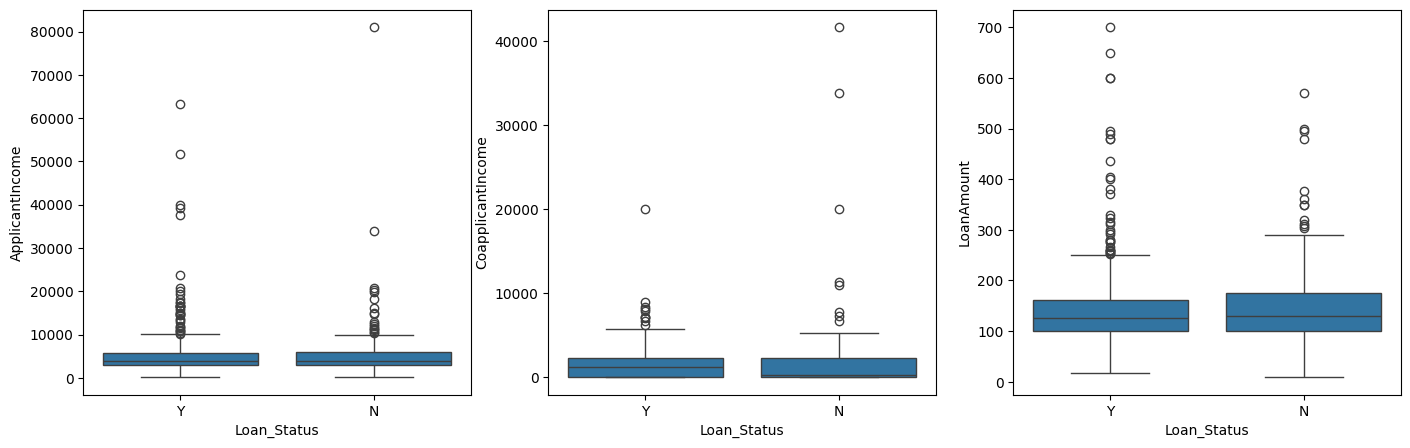
\includegraphics[width=1\linewidth]{Project_Update_Template (1)/outliers.png}
  \caption{Numerical Outliers}
\end{figure}

Feature Engineering. Finally, we used the debt-to-income ratio leveraged by lenders for risk assessment and outlined by Wells Fargo as a base for our improved features \cite{item 12}. The next three influential features were our numerical features: Applicant Income, Co-Applicant Income, and Loan Amount. Therefore, to use these features most effectively, we combined them into $Total\_Income = Applicant\_Income + Co\-Applicant\_Income$, $Monthly\_Payment=$ $ Loan\_Amount$ $/ Loan\_Amount\_Term$, and $Balance\_Income$ $= Total\_Income - Monthly\_Payment$. Now we are ready to train some models.

\section{Training}
Across all models, we first split the data into $75\%$ training data and $25\%$ test data. Then, we performed $5$ cross-fold validation applied to a grid-search to tune the hyper-parameters specific to that model. 

\subsection{Linear Models: Logistic Regression}
For Logistic Regression, we performed additional preprocessing on the dataset. Specifically, we attempted to scale observations through standardization, normalization, and using a robust scaler to keep data within a quantile range. Standardizing the data worked the best as it gave $\approx 1.5\%$ greater accuracy then the robust scaler. Normalizing the data only performed better than no scaling but still performed quite poorly. 

In addition, because each Logistic Regression solver has its own associated loss functions, we had to tune each solver separately which meant performing cross-validation on 6 separate Logistic Regression solvers. In particular we tuned on the regularization parameter C, the l1ratio for the Saga solver, and the solver / loss function used. We also trained the Logistic Regression Model with balanced class weights to mitigate the imbalance of the target label. In the end, all of them performed roughly the same with the two best solvers being Saga with a stronger regularization parameter of $.01$ and $l1\_ratio$ of $.1$ and liblinear with a weaker regularization parameter of $.11$.  

\begin{table}[H]
\centering
  \begin{tabular}{|l|c|l|c|c|} \hline 
 
Solver& Accuracy&  f1-score&C& penalty\\ \hline 

Saga& \textbf{80.7\%}&  \textbf{87.5\%}&.01& elasticnet\\ \hline  
Liblinear&  79.8\%&  86.8\%&.11& l1\\ \hline 
\end{tabular}

 \caption{Logistic Regression}
 \end{table}

All in, Logistic Regression performed fairly well on the dataset after standardizing the values. The Saga solver out-performed the remaining solvers by roughly $1\%$ accuracy but it also cost $40x$ the computation to tune the hyper-parameters so there was some trade-off in using that solver over the faster liblinear alternative. In addition, none of the Logistic Regression solvers seemed able to correctly classify some of the more obscure observations in the dataset. Perhaps SVC will perform better in comparison.

\subsection{Linear Models: Support Vector Machine}
Due to the significant misclassification error of our dataset by the Logistic Regression model, we swayed toward a Support Vector Machine Classifier to see if we could sacrifice misclassifying some outlier data points to achieve higher overall accuracy. For the support vector machine model, we also standardized all of the observations in the same manner as before. In addition, we tuned the regularization (C) hyper-parameter to achieve a good tradeoff between a sufficiently large margin and lower training error. We also tuned the Kernel parameter with a relatively low degree for the polynomial kernel, between 2-8 degrees, because larger degrees seemed to overfit on the tabular data. In the end, the sigmoid kernel vastly outperformed the polynomial and linear kernels and slightly beat out the rbf kernel. The sigmoid kernel did use a relatively weak regularization parameter of $.21$ leading to a wider margin but higher misclassification error. 
\begin{table}[H]
\centering
  \begin{tabular}{|l|c|l|c|c|} \hline 
 
Kernel& Accuracy&  f1-score&C& gamma\\ \hline 

Sigmoid& 80.6\%&  87.3\%&.21& auto\\\hline 
\end{tabular}

 \caption{Support Vector Machine}
 \end{table}

\subsection{Bagging: Extra Trees}
A note on Bagging. All the bagging classifiers were trained using grid-search cross-fold validation on the Bagging Classifier with the base estimator as the underlying classifier to achieve the appropriate variability necessary for Bagging to be effective. 

After the relative success of the linear models on our dataset we decided that bagging a tree model may better capture our features' relationship to Loan Status. For the Extra Trees classifier, we performed hyper-parameter tuning on the number of trees in the forest, the loss function, impurity decrease per split, and the maximum number of features to consider for each split. 

All of the parameters chosen seemed to pretty standard with a relatively low number of trees, only 100, the gini loss function, and log base 2 features examined for each split. In addition, we did not originally bound the impurity decrease but without this, the model quickly overfit on the dataset and continually over-predicted the majority class because we did not control tree depth. 

On the Bagging Classifier, we trained on out-of-bag scoring, bootstrapping features, and a balanced subsample for our class weight. This means that for each tree we add a weight coefficient per feature inversely related to the frequency it appears in the bootstrapped data. This will aid in mitigating the imbalance of the underlying dataset. We also trained on between $10-1000$ Extra-Trees models in the Bagging Classifier but it made a non-negligible difference in accuracy after 100 models. Using 1 model was very overfit on the majority class but even after 10 models there was minimal increase to accuracy.

Unfortunately, despite the additional computational effort to perform Bagging on the Extra Trees classifier, it performed roughly as well as the Support Vector Machine Classifier, and slightly worse than plain Logistic Regression. 

\begin{table}[H]
\centering
  \begin{tabular}{|c|l|c|l|l|} \hline 
 
 Accuracy&  f1-score&Loss& Trees&Extra-Trees\\ \hline 

 80.5\%&  87.5\%&gini& 100&10\\\hline 
\end{tabular}

 \caption{Bagging Extra Trees}
 \end{table}

\subsection{Bagging: Gradient Boosting}
There was little work to do in training the Gradient Boosting Classifier. We tuned on the loss function, scoring criterion, number of estimators, and of course on the number of Gradient Boosting models that we used in the Bagging Classifier. Overall, this classifier was quick to train and performed better than all the models up to this point.

We used 50 Gradient Boosting Classifiers, each of 100 estimators, with Friedman mean squared error to be less sensitive to outliers, and log loss. We also maintained standard practice by allowing for square root features to be examined at each step. 

\begin{table}[H]
\centering
  \begin{tabular}{|c|l|c|l|l|} \hline 
 
 Accuracy&  f1-score&Loss& Trees&GB's\\ \hline 

 81.2\%&  87.7\%&log& 100&50\\\hline 
\end{tabular}

 \caption{Bagging Gradient Boosting}
 \end{table}

Here Gradient Boosting outperformed all of the previous linear and Tree models. However, this was not as significant an improvement as we had hoped to see. It does seem as though the models up to this point have been over-fitting because the training error and testing error have been marginally different, $\approx 2\%$. Therefore, another hypothesis may be that we require a model capable of learning more complex functions. To test this theory, we will examine a neural network classifier next.

\subsection{Neural Network: MLP}
Lastly, we used a Multi-Layer Perceptron (MLP) Classifier in an attempt to learn what may be a much more complex function than what linear models or even trees can capture. The MLP Classifier performed best with a tanh activation function and a constant learning rate. Additionally, it uses the 'sgd' solver for optimization, which is particularly suited for larger datasets and tends to perform better when the number of samples is high. This was interesting as our data-set was relatively small, roughly 400 observations and gradient descent required 400 iterations to converge. In fact, sgd would often not converge even with this high number of iterations. It is also interesting that the Multi-Layer-Perceptron worked best with a tanh activation function which always gives a derivative less than or equal to one, and as such has issues with vanishing gradients. This provides evidence for the efficacy of smaller hidden-layer sizes, 20 layers, and a constant learning rate.

In the end, the best Multi-Layer Perceptron Classifier performed worse than Bagging Gradient boosting but slightly better than the rest of the previous models. We also tuned an MLP Classifier with a logistic activation function which performed slightly worse than the tanh activation function with an accuracy of $80\%$. Due to the performance of the MLP in general and with the logistic activation function, it is not clear that the Loan Prediction dataset requires a complex model to fit the correct function. Instead, it may be the case that the missing data outlined earlier or outliers within the testing data make it challenging to accurately predict the test set with any model. Therefore we argue that Loan prediction does not require a more complex model but simply more processing of the input data to account for these irregularities.

\begin{table}[H]
\centering
  \begin{tabular}{|c|l|c|l|l|} \hline 
 
 Accuracy&  f1-score&Solver& Alpha&Activation\\ \hline 

 80.8\%&  87.5\%&sgd& .0001&constant\\\hline 
\end{tabular}

 \caption{MLP}
 \end{table}


\section{Results}
A Note on Scoring: To score a model, we take the original data-set, and split it into (75\%) train and (25\%) test data. Then train each model on the training data we have split off using the optimal hyper-parameters we found earlier. Finally, we test the model on the split-off test data. We perform this scoring routine over 100 iterations for each model to get aggregate data on f1-score and accuracy. In addition, we have linked the GitHub repository below for those who want to replicate our results or test their own models \footnote{\url{https://github.com/gabrieliUNC/ML_Final_Project}}.

\begin{table}[H]
\centering
  \begin{tabular}{|>{\raggedright\arraybackslash}p{0.15\linewidth}||>{\raggedright\arraybackslash}p{0.2\linewidth}||>{\centering\arraybackslash}p{0.15\linewidth}|>{\raggedright\arraybackslash}p{0.15\linewidth}|} \hline 
 
   Bagging&Model&Accuracy&  f1-score\\ \hline 

   N/A&Logistic Regression&80.7\%&  87.5\%\\\hline
  N/A&SVC& 80.6\%&87.3\%\\\hline
  100&Extra Trees& 80.5\%&87.5\%\\\hline
  100&Gradient Boosting& \textbf{81.2\%}&\textbf{87.7\%}\\\hline
  N/A&MLP& 80.8\%&87.5\%\\\hline 
\end{tabular}

 \caption{Model Scores}
 \end{table}

Based on the accuracy and f1-scores across all the models, it appears that Logistic Regression may be the right fit for predicting Loan Status. It is not clear that applying more complex models garners significant additional knowledge over naive Logistic Regression. Indeed, this can be seen from examining the accuracy and f1-scores of the 5 models we trained, which all fall within $+/-1\%$ of each other. Although Bagging 50 Gradient Boosting models or using a neural network did achieve higher accuracy than the Logistic Regression model, this improvement was meager. The relatively negligible increase in accuracy over Logistic Regression reinforces the claim that Loan prediction may be performed more accurately with a simpler function and more data processing. For example, in the real world, forcing applicants to provide answers to all questions, would likely increase the accuracy of a model which does not have to handle missing data.

\section{Conclusion}
This paper serves as an experimentation of sorts into what classes of models most aptly solve the loan prediction problem. Our focus on understanding and manipulating the underlying dataset to work with each model will allow replication of our work for those who seek to validate or argue the efficacy of the models present in this paper or other ML models. In addition, we argue, that with our loan prediction data, simple is better. There is no need for state-of-the-art prediction when it incurs state-of-the-art cost and a basic model will perform comparably with a smaller computational price tag.

This comprehensive approach to developing a loan prediction model not only enhances the reliability of the predictions but also provides a robust framework that can be adapted for similar problems in financial analytics. This makes this research valuable not just for its immediate application but also as a methodological reference for future studies in the field of credit risk assessment.


\appendices
\section{Supplementary content}
\newline
\begin{figure}[H]
        \centering
        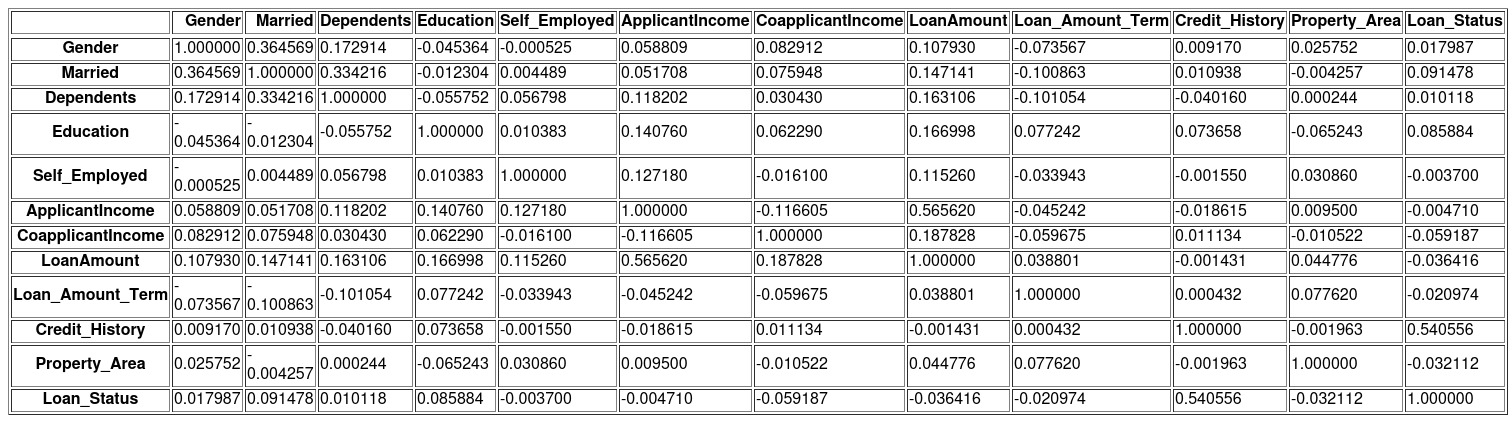
\includegraphics[width=1\linewidth]{Data5.jpg}
        \caption{Correlation Matrix}
        \label{fig:enter-label}
    \end{figure}


\begin{thebibliography}{9}

\bibitem{item1}
M. A. Sheikh, A. K. Goel and T. Kumar, "An Approach for Prediction of Loan Approval using Machine Learning Algorithm," 2020 International Conference on Electronics and Sustainable Communication Systems (ICESC), Coimbatore, India, 2020, pp. 490-494, doi: 10.1109/ICESC48915.2020.9155614.

\bibitem{item2}
Zimmerman, G. (1996), "Factors influencing community bank performance in California. Federal"
Reserve Bank of San Francisco 1: 26-41.

\bibitem{item3}
Anand, M., Velu, A., & Whig, P. "Prediction of Loan Behaviour with Machine Learning Models for Secure Banking" Journal of Computer Science and Engineering (JCSE), 2022, pp. 1–13, doi: https://doi.org/10.36596/jcse.v3i1.237

\bibitem{item4}
Chiang, R.C., Chow, YF. & Liu, M. Residential Mortgage Lending and Borrower Risk: The
Relationship between Mortgage Spreads and Individual Characteristics. The Journal of Real Estate
Finance and Economics 25, 5–32. 2002. https://doi.org/10.1023/A:1015347516812

\bibitem{item5}
Steenackers, A., & Goovaerts, M. J. A credit scoring model for personal loans. Insurance:
Mathematics and Economics. Volume 8, Issue 1, March 1989, Pages 31-34.
https://doi.org/10.1016/0167-6687(89)90044-9

\bibitem{item6}
A. Uzair, T. Aziz, H. Ilyas, S. Asim, B. N. Kadhar, "An Empirical Study on Loan Default Prediction
Models" Journal of Computational and Theoretical Nanoscience, Volume 16, Number 8, August 2019,
pp. 3483-3488(6). DOI: https://doi.org/10.1166/jctn.2019.8312

\bibitem{item7}
L. Zhu, D. Qiu, D. Ergu, C. Ying, and K. Liu, “A study on predicting loan default based on the
random forest algorithm,” Procedia Computer Science, vol. 162, pp. 503–513, 2019, doi:
10.1016/j.procs.2019.12.017

\bibitem{item8}
N. Ghatasheh, “Business Analytics using Random Forest Trees for Credit Risk Prediction: A
Comparison Study”. International Journal of Advanced Science and Technology. Vol.72, pp.19-30.
2014.doi: http://dx.doi.org/10.14257/ijast.2014.72.02

\bibitem{item9}
M. Madaan et al, “Loan default prediction using decision trees and random forest: A comparative
study” IOP Conf. Ser.: Mater. Sci. Eng. 1022 012042. 2021. doi: 10.1088/1757- 899X/1022/1/012042

\bibitem{item10}
Amin R K et al (2015), “Implementation of decision tree using C4.5 algorithm in decision making of
loanapplication by debtor (case study: bank pasar of Yogyakarta special region)”, ICoICT. pp 75–80

\bibitem{item 11}
Chatterjee, Debdatta. “Loan Prediction Problem Dataset.” \textit{Kaggle}, 12 Mar. 2019, www.kaggle.com/datasets/altruistdelhite04/loan-prediction-problem-dataset. 

\bibitem{item 12}
“Calculate Your Debt-to-Income Ratio.” \textit{Calculate Your Debt-to-Income Ratio | Wells Fargo}, www.wellsfargo.com/goals-credit/smarter-credit/credit-101/debt-to-income-ratio/. Accessed 30 Apr. 2024. 


\end{thebibliography}
    

\end{document}
